% Figures for IVF-Bench. Drawn in TikZ/pgfplots so they scale cleanly and carry
% no external image dependency into the arXiv bundle.

% ===== FIG_PIPELINE =====
\begin{figure}[H]
\centering
\begin{tikzpicture}[
  font=\small,
  every node/.append style={execute at begin node=\setlength{\emergencystretch}{2em}},
  box/.style={draw, rounded corners=3pt, align=center, inner sep=5pt,
              minimum height=9mm, text width=#1},
  dec/.style={draw, diamond, aspect=3.2, align=center, inner sep=1pt,
              font=\scriptsize, minimum width=30mm, minimum height=13mm},
  ar/.style={-{Latex[length=2mm]}, thick},
]

% ---- left column: the conventional framing. Explicit y coordinates, so
% nothing can collide as node heights change.
\node[font=\bfseries] at (0,0.9) {Conventional evaluation};
\node[box=28mm] (li) at (0,0)    {Embryo image};
\node[box=28mm] (lm) at (0,-1.6) {Scoring model\\[-1pt]\footnotesize CNN or time-lapse};
\node[box=28mm] (ls) at (0,-3.2) {Scalar score};
\node[box=28mm] (lr) at (0,-4.8) {Ranked embryos};
\node[box=28mm, fill=black!5] (lo) at (0,-6.6) {Scored by outcome\\[-1pt]\footnotesize AUROC only};
\foreach \a/\b in {li/lm, lm/ls, ls/lr, lr/lo} \draw[ar] (\a) -- (\b);

% ---- right column
\node[font=\bfseries] at (7.4,0.9) {IVF-Bench (this work)};
\node[box=54mm] (ri) at (7.4,0)
  {Embryo image \textbf{+} patient context\\[-1pt]
   \footnotesize Gardner grade, cycle data, history};
\node[box=54mm] (rm) at (7.4,-1.7) {Vision-language model};
\node[box=56mm] (ra) at (7.4,-3.2)
  {Open-ended assessment\\[-1pt]
   \footnotesize morphology, integration,\\[-1pt]probability, plan};
\node[dec] (rd) at (7.4,-4.7) {which part?};
\node[box=25mm, minimum height=12mm] (rj) at (5.3,-6.5)
  {Five rubrics\\[-1pt]\footnotesize LLM judge, 1--5};
\node[box=25mm, minimum height=12mm] (rp) at (9.5,-6.5)
  {Stated probability\\[-1pt]\footnotesize Brier, AUROC};
\node[box=54mm, fill=black!5] (ro) at (7.4,-8.3)
  {Scored by rubrics \textbf{and} outcome};

\foreach \a/\b in {ri/rm, rm/ra, ra/rd} \draw[ar] (\a) -- (\b);
\draw[ar] (rd.west) -- ++(-2.1,0) node[midway, above, font=\scriptsize] {reasoning} |- (rj.north);
\draw[ar] (rd.east) -- ++(2.1,0)  node[midway, above, font=\scriptsize] {prognosis} |- (rp.north);
\draw[ar] (rj.south) -- ($(ro.north west)!0.5!(ro.north)$);
\draw[ar] (rp.south) -- ($(ro.north east)!0.5!(ro.north)$);
\end{tikzpicture}
\caption{Conventional embryo-selection evaluation against IVF-Bench. Prior work
maps an image to a scalar and is scored only by how well that scalar ranks
outcomes, so a system that reasons well about a patient and one that does not are
indistinguishable. IVF-Bench supplies the patient context alongside the image,
elicits an open-ended assessment, and scores the reasoning against five clinical
rubrics while separately scoring the stated probability against the recorded
outcome.}
\label{fig:pipeline}
\end{figure}

% ===== FIG_RUBRICS =====
\begin{figure}[H]
\centering
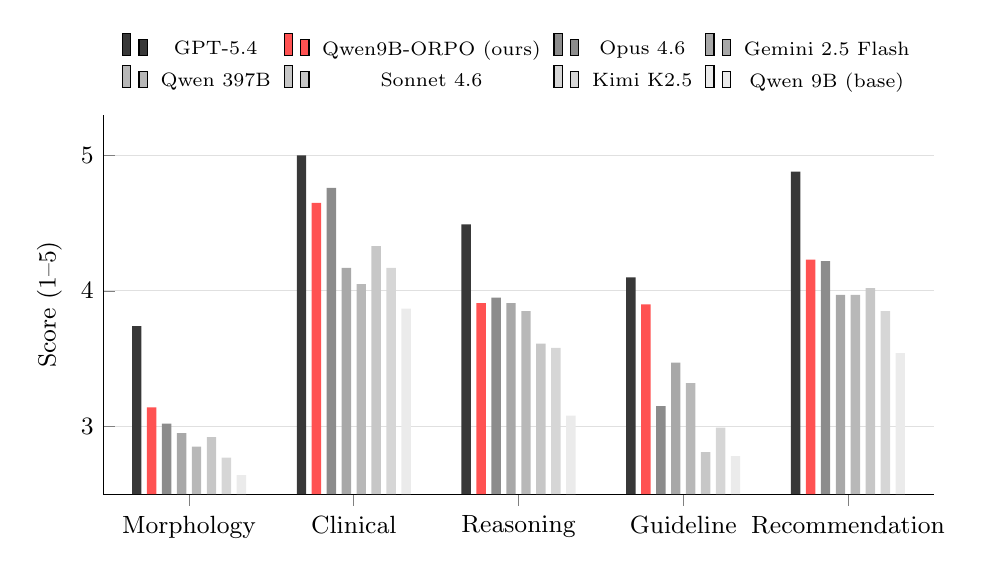
\begin{tikzpicture}
\begin{axis}[
  width=\textwidth, height=6.4cm,
  ybar, bar width=3.4pt,
  ymin=2.5, ymax=5.3,
  ylabel={Score (1--5)}, ylabel style={font=\small},
  symbolic x coords={Morphology,Clinical,Reasoning,Guideline,Recommendation},
  xtick=data, x tick label style={font=\small},
  y tick label style={font=\small},
  legend style={font=\scriptsize, at={(0.5,1.03)}, anchor=south, legend columns=4,
                draw=none, column sep=0.6ex},
  enlarge x limits=0.13,
  ymajorgrids, grid style={black!12},
  axis lines*=left,
]
\addplot[fill=black!78, draw=none] coordinates {(Morphology,3.74)(Clinical,5.00)(Reasoning,4.49)(Guideline,4.10)(Recommendation,4.88)};
\addplot[fill=red!68, draw=none] coordinates {(Morphology,3.14)(Clinical,4.65)(Reasoning,3.91)(Guideline,3.90)(Recommendation,4.23)};
\addplot[fill=black!45, draw=none] coordinates {(Morphology,3.02)(Clinical,4.76)(Reasoning,3.95)(Guideline,3.15)(Recommendation,4.22)};
\addplot[fill=black!34, draw=none] coordinates {(Morphology,2.95)(Clinical,4.17)(Reasoning,3.91)(Guideline,3.47)(Recommendation,3.97)};
\addplot[fill=black!28, draw=none] coordinates {(Morphology,2.85)(Clinical,4.05)(Reasoning,3.85)(Guideline,3.32)(Recommendation,3.97)};
\addplot[fill=black!22, draw=none] coordinates {(Morphology,2.92)(Clinical,4.33)(Reasoning,3.61)(Guideline,2.81)(Recommendation,4.02)};
\addplot[fill=black!16, draw=none] coordinates {(Morphology,2.77)(Clinical,4.17)(Reasoning,3.58)(Guideline,2.99)(Recommendation,3.85)};
\addplot[fill=black!8, draw=none] coordinates {(Morphology,2.64)(Clinical,3.87)(Reasoning,3.08)(Guideline,2.78)(Recommendation,3.54)};
\legend{GPT-5.4, Qwen9B-ORPO (ours), Opus 4.6, Gemini 2.5 Flash, Qwen 397B, Sonnet 4.6, Kimi K2.5, Qwen 9B (base)}
\end{axis}
\end{tikzpicture}
\caption{Per-rubric scores on the held-out split, graded by a judge that sees the
embryo. Clinical integration is the strongest rubric for every system and
morphology grounding the weakest for seven of eight, the two separated by roughly
1.4 points on average, a pattern that holds across three orders of magnitude in
model size. No rubric is degenerate: each spreads the eight systems across
between 1.1 and 1.4 points, so all five carry information about which system is
which even though they correlate. Our post-trained 9B model tracks the frontier
systems on every rubric and comes closest to GPT-5.4 on guideline alignment,
where it trails by 0.19 points.}
\label{fig:rubrics}
\end{figure}

% ===== FIG_ABLATION =====
\begin{figure}[H]
\centering
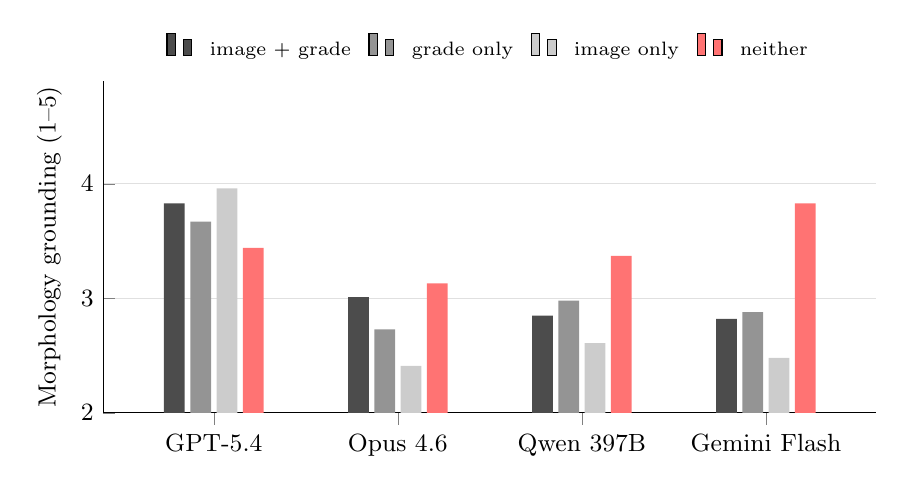
\begin{tikzpicture}
\begin{axis}[
  width=0.94\textwidth, height=5.8cm,
  ybar, bar width=7.5pt,
  ymin=2.0, ymax=4.9,
  ylabel={Morphology grounding (1--5)}, ylabel style={font=\small},
  symbolic x coords={GPT-5.4,Opus 4.6,Qwen 397B,Gemini Flash},
  xtick=data, x tick label style={font=\small},
  y tick label style={font=\small},
  legend style={font=\scriptsize, at={(0.5,1.03)}, anchor=south, legend columns=4,
                draw=none, column sep=1ex},
  enlarge x limits=0.2,
  ymajorgrids, grid style={black!12},
  axis lines*=left,
  % values are in Table~\ref{tab:ablation} directly above; printing them on four
  % adjacent bars collides at this width
]
\addplot[fill=black!70, draw=none] coordinates {(GPT-5.4,3.83)(Opus 4.6,3.01)(Qwen 397B,2.85)(Gemini Flash,2.82)};
\addplot[fill=black!42, draw=none] coordinates {(GPT-5.4,3.67)(Opus 4.6,2.73)(Qwen 397B,2.98)(Gemini Flash,2.88)};
\addplot[fill=black!20, draw=none] coordinates {(GPT-5.4,3.96)(Opus 4.6,2.41)(Qwen 397B,2.61)(Gemini Flash,2.48)};
\addplot[fill=red!55, draw=none] coordinates {(GPT-5.4,3.44)(Opus 4.6,3.13)(Qwen 397B,3.37)(Gemini Flash,3.83)};
\legend{image + grade, grade only, image only, neither}
\end{axis}
\end{tikzpicture}
\caption{The two-by-two on morphology grounding, with the judge shown the embryo
in every arm. The red bar is the arm in which the model received neither the
image nor the Gardner grade, and for three of the four systems it is the
\emph{highest} bar, because a model with no inputs declines to describe the
embryo and the rubric scores an honest refusal as a middling success rather than
as a failure. That is why this design cannot measure the image's contribution by
subtraction, and why we retract the quantitative claim an earlier version of this
paper made from it. Section~\ref{sec:ablation} gives the one edge that survives.}
\label{fig:ablation}
\end{figure}

% ===== FIG_BASERATE =====
\begin{figure}[H]
\centering
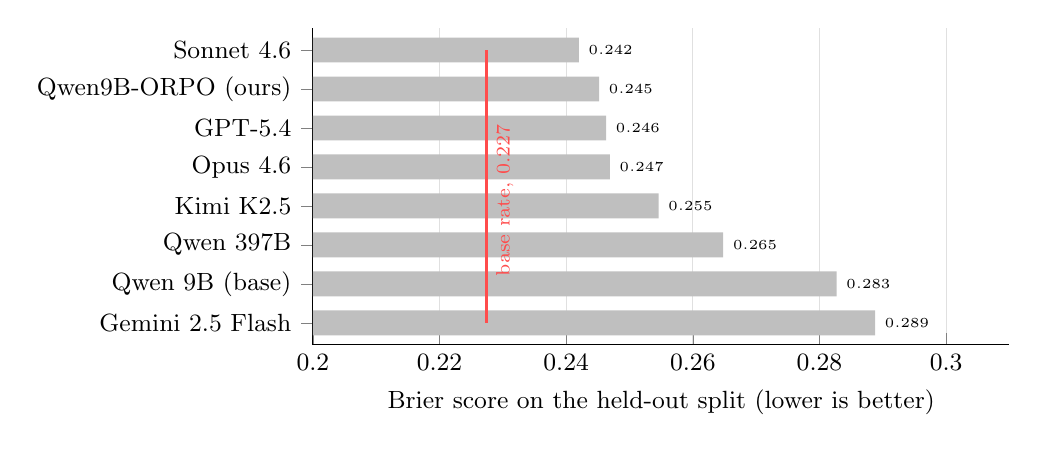
\begin{tikzpicture}
\begin{axis}[
  width=0.86\textwidth, height=5.6cm,
  xbar, bar width=9pt,
  xmin=0.20, xmax=0.31,
  xtick={0.20,0.22,0.24,0.26,0.28,0.30},
  xlabel={Brier score on the held-out split (lower is better)}, xlabel style={font=\small},
  % pgfplots cannot parse parentheses inside a symbolic coordinate, so the
  % display names are supplied separately through yticklabels
  symbolic y coords={Gemini 2.5 Flash,Qwen 9B base,Qwen 397B,Kimi K2.5,Opus 4.6,GPT-5.4,Qwen9B-ORPO ours,Sonnet 4.6},
  ytick=data,
  yticklabels={Gemini 2.5 Flash,Qwen 9B (base),Qwen 397B,Kimi K2.5,Opus 4.6,GPT-5.4,Qwen9B-ORPO (ours),Sonnet 4.6},
  y tick label style={font=\small},
  x tick label style={font=\small},
  xmajorgrids, grid style={black!12},
  axis lines*=left,
  enlarge y limits=0.08,
  nodes near coords, nodes near coords style={font=\tiny, /pgf/number format/fixed,
                                              /pgf/number format/precision=3},
]
% one series only: a second \addplot would make pgfplots group the bars and
% offset every one of them from its category label
\addplot[fill=black!25, draw=none] coordinates {(0.2888,Gemini 2.5 Flash) (0.2827,Qwen 9B base) (0.2648,Qwen 397B) (0.2546,Kimi K2.5) (0.2469,Opus 4.6) (0.2463,GPT-5.4) (0.2452,Qwen9B-ORPO ours) (0.2420,Sonnet 4.6)};
\draw[red!70, very thick] (axis cs:0.2274,Gemini 2.5 Flash) -- (axis cs:0.2274,Sonnet 4.6);
\node[red!70, font=\scriptsize, anchor=north, rotate=90, xshift=2pt]
  at (axis cs:0.2274,Kimi K2.5) {base rate, 0.227};
\end{axis}
\end{tikzpicture}
\caption{Brier score of every evaluated system against a constant predictor that
returns the cohort's clinical pregnancy rate of 0.350 for every case, ignoring
the embryo, the image, and the patient. No system reaches the constant, shown as
the vertical line. We attribute this to the absence of outcome-linked patient
context in the available data rather than to model capacity, for the reason given
in Section~\ref{sec:synthetic}.}
\label{fig:baserate}
\end{figure}
